\section{Proposed Software Architecture}
\subsection{Subsystem Decomposition}
\begin{figure}[H]
	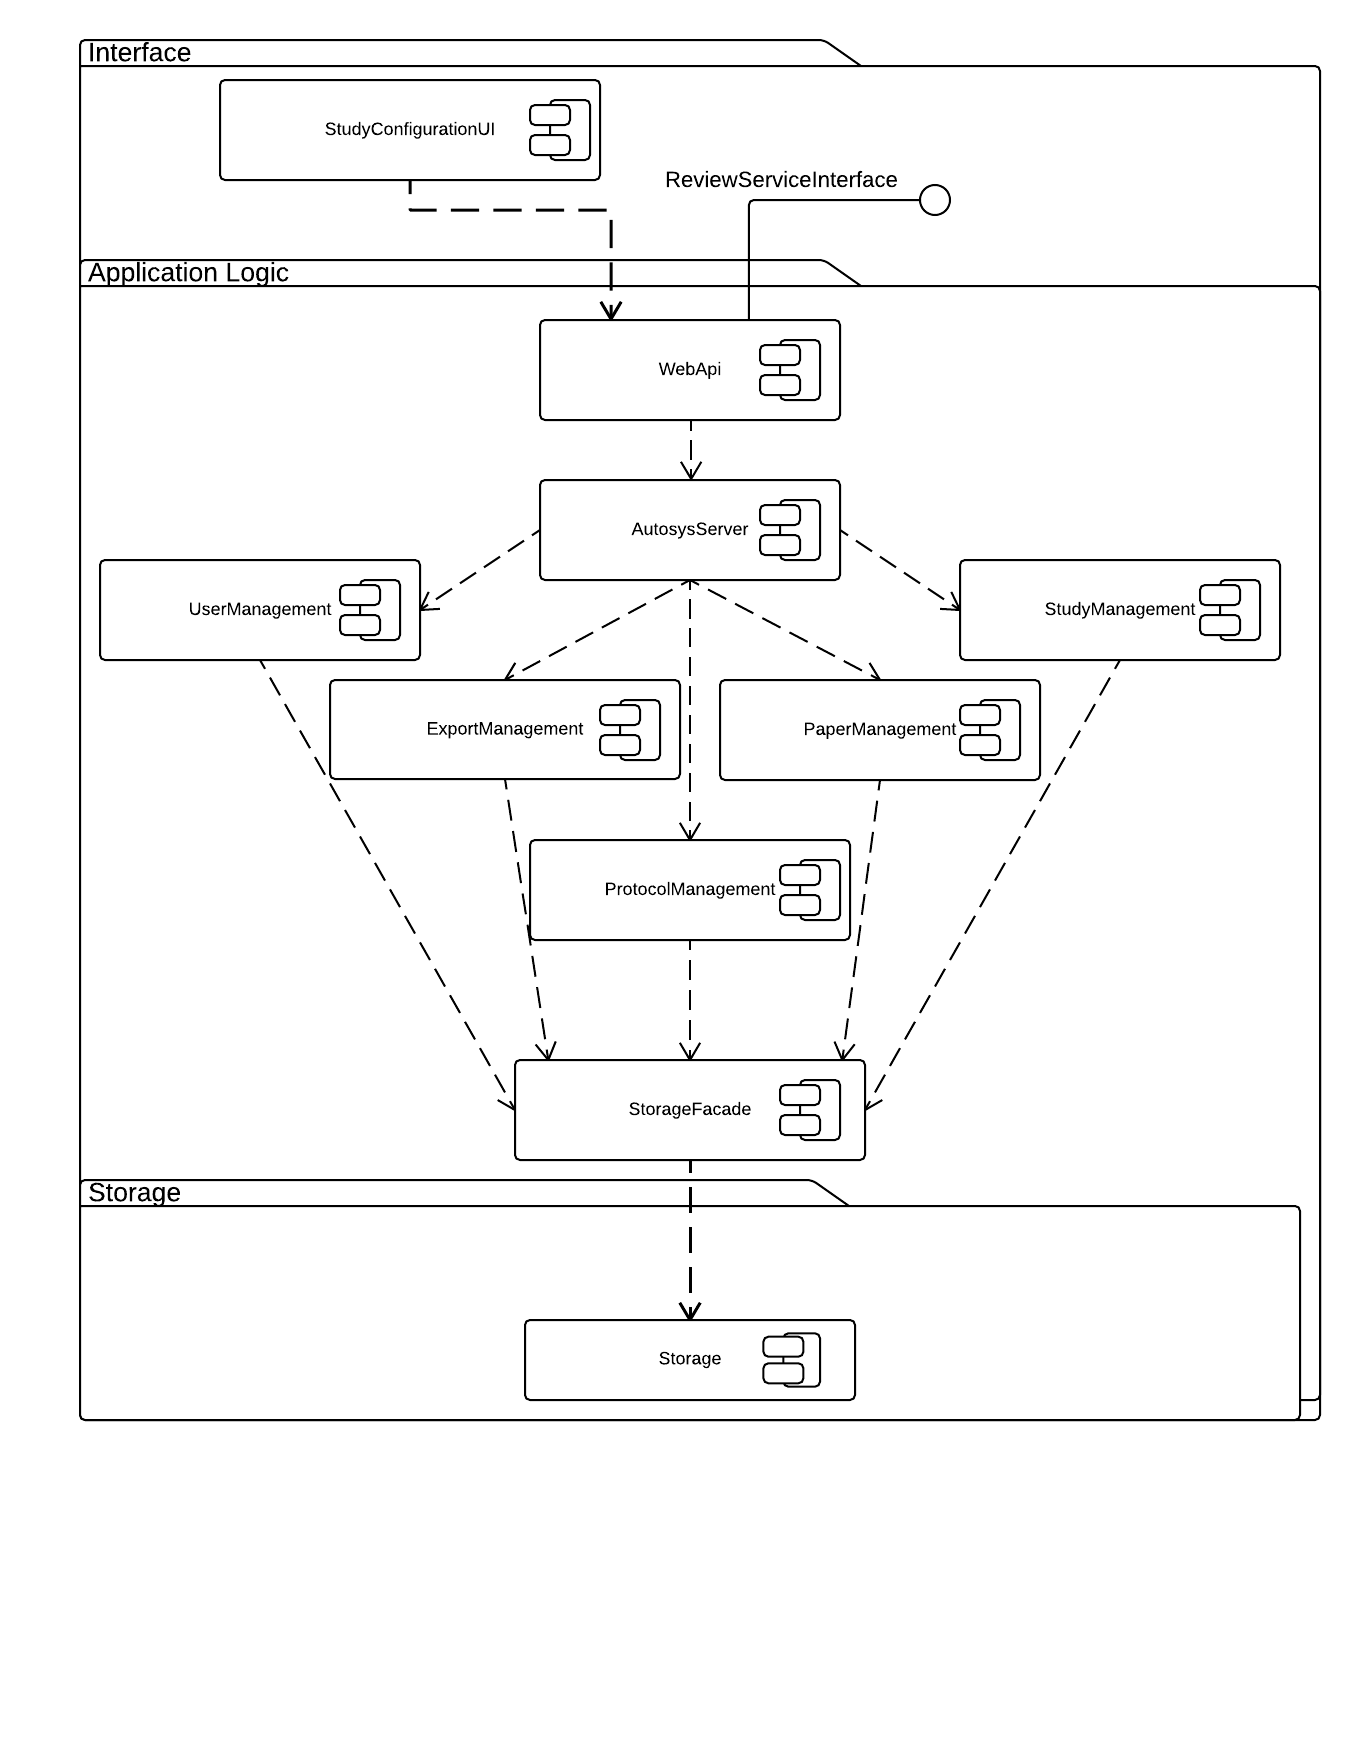
\includegraphics[width = \linewidth]{UMLComponentDiagramSubsystems}
	\caption{Autosys subsystem decomposition (UML Component Diagram, layers shown as UML packages)}
	\label{fig:Subsystem Decomposition, UML Component Diagram}
\end{figure}
As it can be seen on the figure above a three-tier architectural style has been used for the decomposition of the system. The resason for this architecture instead of the two-tier client/server style is that, client/server has a tendency to closly combine the application data and application logic on the server. By using a three-tier style the devision into independent tiers for Interface, Application Logic, and Storage makes it possible to update or change the individual tiers without affecting the whole application. In this way the scaling and managment of the system becomes more flexible than by just using a client/server architectural style.
Also it is woth noting that you still get the possibility for high security, and easier administration of the data, through a centralized data access.\\
From the functional requirements of the Autosys RAD document the following needed services are defined by grouping related operations that share a common purpose:\\
\begin{itemize}
	\item Study Configuration
	\item Task Handling
	\item Paper Screening
	\item Study Export
	\item User Validation
	\item User Management
	\item Research Protocol Generation
\end{itemize}
The \textbf{StudyConfigurationClient} provides the configuration of studies service. It is a front end for users to initiate all use cases related to setting up or configuring a \textbf{Study}.
The \textbf{ReviewService} provides an interface for different Review Clients to communicate with the \textbf{AutosysServer}, such that the system is not depenendt on the review client which makes the design more flexible.
The \textbf{AutosysServer} will be providing the user validation services for allowing users access to other of the components in the application logic. 
The \textbf{UserManagement} component is providing the user management service, since it holds the responsibility for handling all CRUD operations regarding teams and individual users. The \textbf{StudyManagement} component  provides the study configuration service by allowing users to set up and manage studies information.
The \textbf{ExportMangement} is doing study export services which consist of exporting Studies as plain data sets such as cvs files.
The \textbf{PaperManagement} provides the paper screening service, as it runs the filtering mechanisms on the research papers to get relevant papers according to the Study Criteria and Classifications.
For the Research Protocol Generation service the component \textbf{ProtocolManagement} is created, which will be managing the export of protocols for studies based on the study's configuration.
The\textbf{ Storage} interface is used for a Bridge Pattern to decouple the storage abstraction from the application logic so that the two can vary independently. At the bottom tier the \textbf{AutosysStorage} represents the subsystem for storing the user data, study data, and research papers.

\subsection{Identifying and Storing Persistent Data}
\paragraph{Identifying persistent objects}\mbox{}\\

Autosys deals with three sets of objects that must be stored.  The first set (referred as metadata storage) consists of research data such as metadata on articles which are accessed during conduction of secondary studies. The second set (referred as blue storage) consists of objects that are created and accessed by the blue part of the system(eg. Users, roles, etc). It needs to be persistent to track the progress of the study and who is involved. The third set (referred as configuration storage) consists of data for a study configuration that are created by the study configuration UI. The data defines the study configuration such as research questions, tasks, inclusion and exclusion criterias etc.\\\\ 

Metadata storage is well defined and will rarely change during the lifetime of Autosys. These changes may occur whenever new research data has been created or removed and thus create a need for an update of the set. Objects within blue storage are managed and defined by the blue part of the system. Hence, we decide to let the blue part decide how to manage and access these persistent object through a generic interface. Configuration storage is also well defined and will not change once the study configuration has been made.

In this scope of the Autosys system, the main focus of persistent objects is set on metadata storage and configuration storage.

\paragraph{Selecting a storage strategy}\mbox{}\\
By selecting and defining a persistent storage, strategy enables us to deal with issues related to storage management. The main design goals of the yellow part of Autosys is to be reliable, scalable while also has high performance. It is therefore decided to implement a database management system since it allows concurrent queries and provide transaction mechanisms to ensure data integrity. \\\\Compared to a flat file storage method, a database management system will also scale to large installations with many researchers that are to conduct studies simultaneously. However, to allow future upgrades or changes it has been decided that the storage strategy is not solely dependent on a database management system. Thus, the storage subsystem will provide an abstract interface that enables other kinds of storage to be coupled. The users of Autosys are not able to change the storage, however if an update is ever needed for the storage strategy, a system administrator are able to do so. 

\subsection{Providing Access Control}
This section aims to show how the yellow system handles requests from clients based on which actor they represent. AutoSys is a multi-user system with a manager and researcher actor. A researcher can both be assigned the role of a reviewer and validator since only their tasks are different. We have drawn an access control matrix depicting the allowed operations on the entity objects for both actors. In summary, a Manager can create Users and Teams while Researchers can create Studies and receive Tasks. Ideally, all actors must first authenticate based on their role before they can modify any object in the system. One would then use access control lists on each object to check the access privileges of the user. 
Below is the access matrix for main AutoSys objects. Note that the study object is comprised of a StudyReport, ResearchProtocol and a Phase with Criteria. Tasks are generated in a Phase. Also, we have omitted method names for Users and Teams that only have CRUD operations. Finally, we assume that a Manager cannot also be a Researcher. 

\begin{figure}[H]
	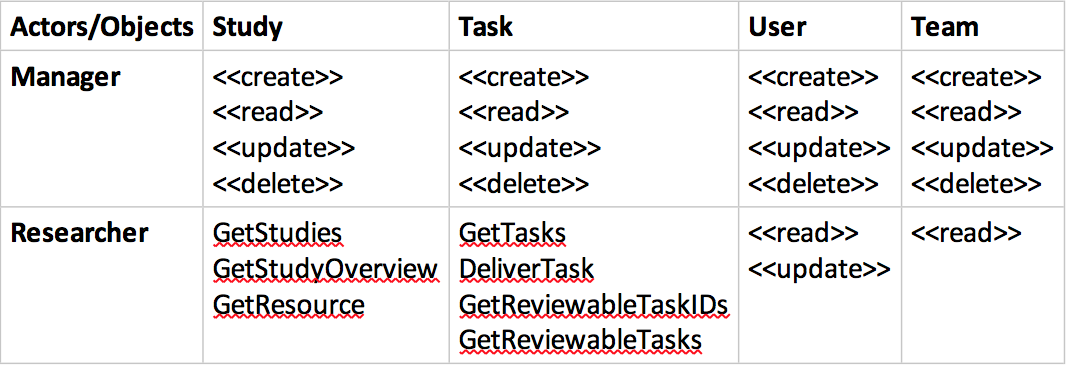
\includegraphics[width = \linewidth]{Images/accessmatrix}
	\caption{Access matrix for main AutoSys objects}
	\label{fig:accessmatrix}
\end{figure}

\subsection{Designing the Global Control Flow}
When selecting components for the interface and storage subsystems of Autosys, we effectively narrowed the alternatives for control flow mechanisms for the yellow part of Autosys. The autosysStorage is located in a web server. The web server awaits requests from the blue part of autosys or the studyConfigurationUI. For each request the web server receives, a new thread is made, which enable the web server to parallel handling of the requests. This results in a more responsive system. By example, the web server can process and handle a given process x while another process awaits a respond from the database. However, the stumbling block of threads is the increased complexity of the system resulting from the usage of threads. To establish a sturdy design with concurrency taken into consideration, one will define the following strategy for dealing with concurrent accesses to the shared storage:
\begin{itemize}
	\item \textit{Boundary objects should not define any fields.} Boundary objects should only hold temporary data correlated with the current request in a local variable.
	\item \textit{Entity objects should not provide direct access to their fields.} All changes and accesses to a given object state should be done through dedicated methods. 
	\item \textit{Methods for accessing state in entity objects should be syncronized}. By using thread synchronization mechanism provided by C#, only one thread can be active at a time in an access method.
	\item \textit{Nested calls to synchronized methods should be avoided.} When creating synchronized methods, one must make sure if a nested method call can lead into calling another synchronized method. The reason for this is to avoid deadlocks and must be avoided. If nested calls are unavoidable, one should either relocate the logic among methods to or impose a strict ordering of synchronized method calls.
	\item \textit{Redundant state should be time-stamped} The state of an object can periodically, be duplicated. By example, two researchers may create objects with the same state and can lead to conflicts. To avoid this, objects should be time-stamped or have another unique identifier.

\end{itemize}


\subsection{Hardware/Software mapping}
\paragraph{Systems}\mbox{}\\
This program is inherently a documentation tool which map research articles goals and conclusions in a searchable context. This requires the program to be stable and reliable, especially  in the context of data preservation. \\The program is split in two components, a client and a external database  server. The user will run a client on his computer which will communicate with the server which runs the application logic and storage. The user client will feature data preservation, to enable offline functionality, but only to a limited extend. This report primarily focus on the server, if any questions to the user client should occur,  please refer to the according Blue SDD.\\ \\
All user clients will contact the a single server. To solve this, the server will be multi threaded, which allows for multiple users interacting with the server at the same time, but  At the current scope of the program, this is possible due to low amount of users, but should this system expand a new design should be conceived. \\
\begin{figure}[H]
	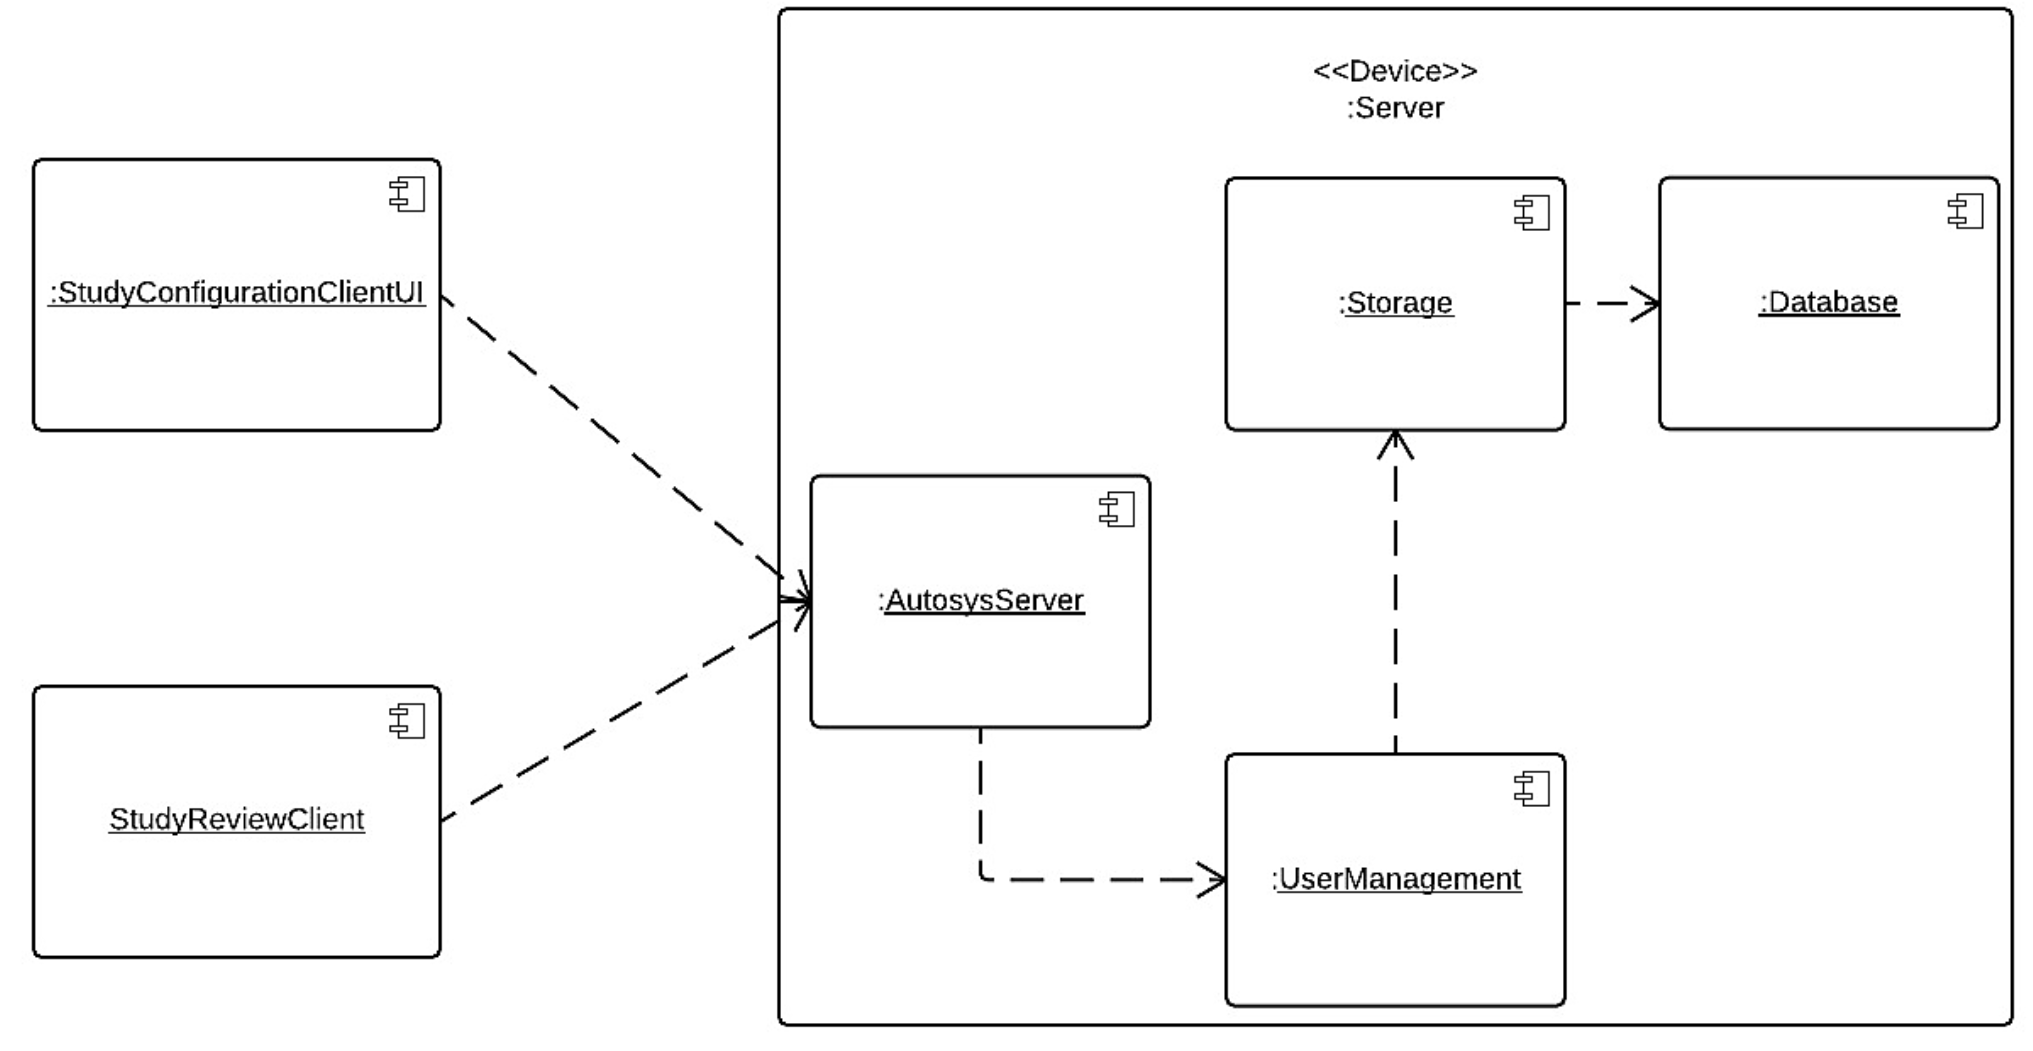
\includegraphics[width=\textwidth]{mappingImage}
	\caption{ Software mapping of prior subsystem decomposition. Note that the components UserManagement, PaperManagement and StudyManagement has been collapsed into a single unit called UserManagement }
\end{figure}
\paragraph{Program components}\mbox{}\\
The server will be implemented in C Sharp as requested by the the client. By using C Sharp, we can utilise to Microsoft expansive database systems and interfaces especially in regards to the database. Additionally this also make the program easier to maintain, since C Sharp is a well known language and can utilise the .NET framework. As communication between the server and the clients, we plan to communicate with HTTPS  request containing JSON object. This will make it easier to implement future changes and even completely replace the clients user interface with a more modern solution like a web page
\\\\
To achieve fast database responses, we will implement an entity framework database, which utilizes Microsoft?s .NET framework to optimize database queries. This takes advantage of optimized queries and features implemented by Microsoft database experts. Furthermore, a future feature may be implemented to cache the result of large queries for quick access. This allows the server to respond hastily to large queries, which have previously been used. This will only be implemented for queries on data that is less likely to change. As a result, a memory trade-off may occur, which can be negated by using limits on how much memory and how many queries are cached. By way of example, the last x number of query results to the server could be cached for repeated use. The design goal is a refinement of the non-functional requirement ?high performance? in the Requirement Analysis Document.